\documentclass{article}
\usepackage[utf8]{inputenc}
\usepackage{amsmath}
\usepackage{amssymb}
\usepackage{tikz}
\usepackage{xeCJK}

\begin{document}

\noindent \textbf{P13.2.} 将工厂抽象为一个 9 个顶点的无向图，业务联系即为边。则
\begin{enumerate}
    \item 每座工厂只与其他 3 座工厂有业务联系，即每个点的度数都为 3（奇数）。根据握手定理，奇度点的个数不可能是奇数个（一共 9 个），所以不成立；
    \item 同理，第二个中表示着有 5 座工厂与奇数个工厂有业务联系，即 5 个奇度点，也不成立。
\end{enumerate}

\noindent \textbf{P13.4.} 考虑最简单的反例：假设有 1 个孤立顶点，除去这个点的子图是全联通的完全图，这时出现最多有 $\sum_{i=1}^{n-2}i=\frac{(n-2)(n-1)}{2}$ 条边。然而 $m > \frac{(n-2)(n-1)}{2}$，所以该图不存在孤立顶点。

\noindent \textbf{P13.7.} 假设共有 $n$ 个点，显然对于任意一个点 $v_i$，$d^+(v_i)+d^-(v_i)=n-1,\sum_{v_i \in V}d^+(v_i)=\sum_{v_i \in V}d^-(v_i)=|E|=\frac{n(n-1)}{2}$。\\
那么
\begin{align*}
&\sum_{v_i \in V}(d^+(v_i))^2-\sum_{v_i \in V}(d^-(v_i))^2 \\
&=\sum_{v_i \in V}(d^+(v_i))^2-\sum_{v_i \in V}[(n-1)-d^+(v_i)]^2 \\
&=\sum_{v_i \in V}(d^+(v_i))^2-[n(n-1)^2+\sum_{v_i \in V}(d^+(v_i))^2-2(n-1)\sum_{v_i \in V}d^+(v_i)] \\
&=2(n-1)\sum_{v_i \in V}d^+(v_i)-n(n-1)^2\\
&=n(n-1)^2-n(n-1)^2\\
&=0
\end{align*}
所以 $\sum_{v_i \in V}(d^+(v_i))^2=\sum_{v_i \in V}(d^-(v_i))^2$

\noindent \textbf{P13.8.} 
% 此处原为图片占位

\noindent \textbf{P13.10.}

% 第一个 SVG 的 TikZ 等效实现
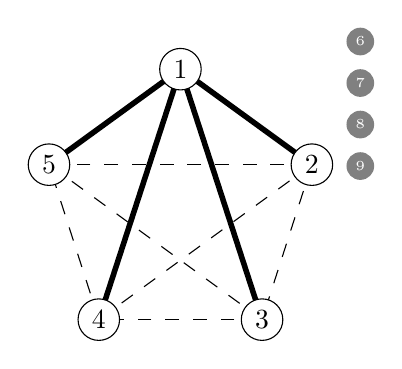
\begin{tikzpicture}[x=0.5pt,y=0.5pt,yscale=-1,xscale=1]
\draw [line width=2] (150,50) -- (245,119);
\draw [line width=2] (150,50) -- (209,231);
\draw [line width=2] (150,50) -- (91,231);
\draw [line width=2] (150,50) -- (55,119);
\draw [dash pattern={on 5 off 5}] (245,119) -- (209,231);
\draw [dash pattern={on 5 off 5}] (245,119) -- (91,231);
\draw [dash pattern={on 5 off 5}] (245,119) -- (55,119);
\draw [dash pattern={on 5 off 5}] (209,231) -- (91,231);
\draw [dash pattern={on 5 off 5}] (209,231) -- (55,119);
\draw [dash pattern={on 5 off 5}] (91,231) -- (55,119);
\filldraw [fill=white, draw=black] (150,50) circle (15); \node at (150,50) {1};
\filldraw [fill=white, draw=black] (245,119) circle (15); \node at (245,119) {2};
\filldraw [fill=white, draw=black] (209,231) circle (15); \node at (209,231) {3};
\filldraw [fill=white, draw=black] (91,231) circle (15); \node at (91,231) {4};
\filldraw [fill=white, draw=black] (55,119) circle (15); \node at (55,119) {5};
\filldraw [fill=gray, draw=none] (280,30) circle (10); \node [white] at (280,30) {\tiny 6};
\filldraw [fill=gray, draw=none] (280,60) circle (10); \node [white] at (280,60) {\tiny 7};
\filldraw [fill=gray, draw=none] (280,90) circle (10); \node [white] at (280,90) {\tiny 8};
\filldraw [fill=gray, draw=none] (280,120) circle (10); \node [white] at (280,120) {\tiny 9};
\end{tikzpicture}

\vspace{1em}

% 第二个 SVG 的 TikZ 等效实现
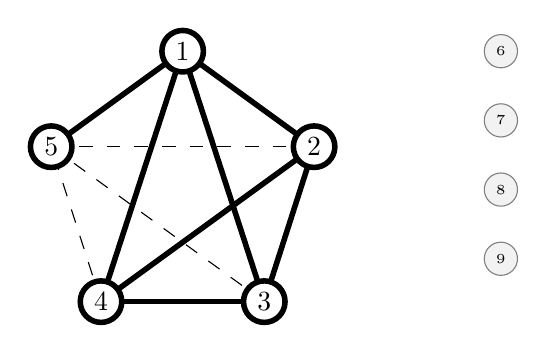
\begin{tikzpicture}[x=0.5pt,y=0.5pt,yscale=-1,xscale=1]
\draw [line width=2] (150,50) -- (245,119);
\draw [line width=2] (150,50) -- (209,231);
\draw [line width=2] (150,50) -- (91,231);
\draw [line width=2] (150,50) -- (55,119);
\draw [line width=2] (245,119) -- (209,231);
\draw [line width=2] (245,119) -- (91,231);
\draw [line width=2] (209,231) -- (91,231);
\draw [dash pattern={on 5 off 5}] (245,119) -- (55,119);
\draw [dash pattern={on 5 off 5}] (209,231) -- (55,119);
\draw [dash pattern={on 5 off 5}] (91,231) -- (55,119);
\filldraw [fill=white, draw=black, line width=2] (150,50) circle (15); \node at (150,50) {1};
\filldraw [fill=white, draw=black, line width=2] (245,119) circle (15); \node at (245,119) {2};
\filldraw [fill=white, draw=black, line width=2] (209,231) circle (15); \node at (209,231) {3};
\filldraw [fill=white, draw=black, line width=2] (91,231) circle (15); \node at (91,231) {4};
\filldraw [fill=white, draw=black, line width=2] (55,119) circle (15); \node at (55,119) {5};
\begin{scope}[shift={(380,50)}]
\filldraw [fill=gray!10, draw=gray] (0,0) circle (12); \node at (0,0) {\tiny 6};
\filldraw [fill=gray!10, draw=gray] (0,50) circle (12); \node at (0,50) {\tiny 7};
\filldraw [fill=gray!10, draw=gray] (0,100) circle (12); \node at (0,100) {\tiny 8};
\filldraw [fill=gray!10, draw=gray] (0,150) circle (12); \node at (0,150) {\tiny 9};
\end{scope}
\end{tikzpicture}

\medskip
本质上是 $R(4,3)$ 的证明。如图，认识为实线边，不认识为虚线边，考虑上面的最简单情况（至少有 1 个点有至少 4 条实线边），此时除非有 4 个人及以上相互认识全为实边，否则一定会存在至少 1 个虚线三角形，即 3 个人相互不认识。

\end{document}
